\documentclass{article}[12pt]
\usepackage{amsmath}
\usepackage{gensymb}
\usepackage{standalone}
\usepackage{verbatim}
\usepackage[utf8]{inputenc}
\usepackage{setspace}
\usepackage[a4paper,margin=1in,footskip=0.25in]{geometry}
\usepackage{graphicx}
\usepackage{mathptmx}
\usepackage{booktabs}
\usepackage{cite}
\usepackage[english]{babel}
\usepackage[utf8]{inputenc}

\begin{document}
\section{Results}
Having verified the functionality of the code, a three terminal device was simulated. The device was $100\mu m$ square with $100$ nodes an each axis. The first terminal was placed on the bottom of the plate and spanned $100\mu m$ at a potential of 30V.  The second terminal was located a $y=100\mu m$ and spanned $30\mu m$ in the postive x-direction at a potential of 100V. The last terminal was located at $y=100\mu m$ and $x=70\mu m$ and spanned $30 \mu m$ at a potential of 0V. The resulting contour plot is seen in Figure \ref{fig:three_terminal}.
\begin{figure}[h!]
	\centering
	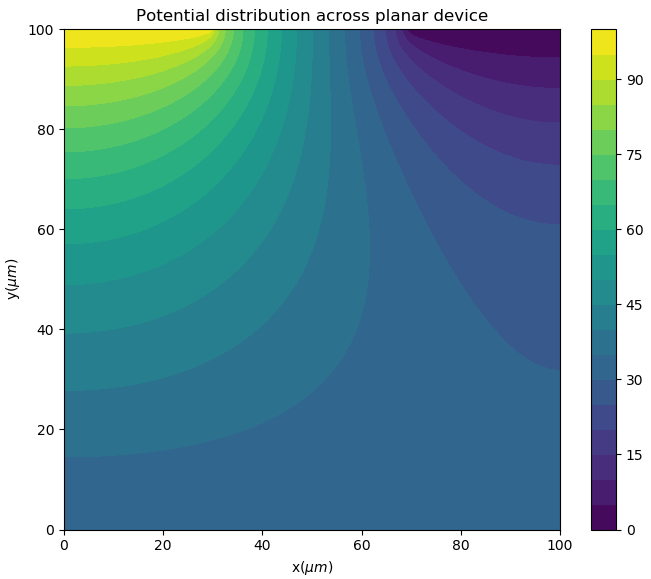
\includegraphics[width=\linewidth]{three_terminal.png}
	\caption{Simulated applied voltage of three terminal device detector geometry.}
	\label{fig:three_terminal}
\end{figure}
\end{document}
